\chapter{Evaluation}
\label{chap:07_evaluation}

In this chapter, the implementation of \Chap{chap:06_implementation} is evaluated in various experiments. Further, the experimental results are summarised and discussed.

\section{Experimental Environment}
%
The experiments are conducted on the DGX introduced in \Sec{sec:06_impl-env}.
% 2 GPUs
As for the implementation, 2 \hyperlink{abbr:gpu}{GPUs} have been available for the experiments.


% ===========================================
% ===========================================
\section{Experiments}
% Intro
The performance of the computing environment is measured on two widely used machine learning algorithms.
% Explain
In both experiments, a machine learning model is trained on the computing environment using Apache Spark. Furthermore, each benchmark is evaluated using three different configurations:
\begin{enumerate}
\item Using a static number of \hyperlink{abbr:cpu}{CPU}-only Apache Spark workers (\Sec{sec:07_static})
\item Using a static number of \hyperlink{abbr:gpu}{GPU}-accelerated Apache Spark workers (\Sec{sec:07_gpu})
\item Dynamically scaling the replicas of CPU-only Apache Spark workers using the \textit{Auto-Scaler} (\Sec{sec:07_auto-scaler})
\end{enumerate}
% 10 times
For each configuration, the experiment is conducted ten times. The spark-job execution time mean value over all ten iterations per experiment is used as the result.
% DIfference between GPU and CPU
The performance difference between \hyperlink{abbr:gpu}{GPU}-accelerated worker nodes, and \hyperlink{abbr:cpu}{CPU}-only worker nodes are explored using a \hyperlink{abbr:cpu}{CPU}-only and a \hyperlink{abbr:gpu}{GPU}-only version of the benchmark implementation.

\paragraph{}
% Why no auto gpu
The \textit{Auto-Scaler} is not evaluated using \hyperlink{abbr:gpu}{GPU}-accelerated worker nodes. As mentioned, for this experiment, only 2 \hyperlink{abbr:gpu}{GPUs} are available. The RAPIDS plugin allocates a \hyperlink{abbr:gpu}{GPU} exclusively for each executor. When the \textit{Auto-Scaler} creates a new worker node, the worker allocates a random available GPU.
% Live system
However, the host machine is a live system. It is not possible to allocate a random \hyperlink{abbr:gpu}{GPU} that may be in use by another application. Furthermore, the \textit{Auto-Scaler} does not support allocating a specific \hyperlink{abbr:gpu}{GPU} for each newly created worker. An approach to overcome this problem is introduced in \Sec{subsec:08_outlook_gpus}.

\paragraph{}
% The algorithm
The two benchmarks to evaluate the performance are:
\begin{itemize}
\item XGBoost classification model using the \textit{Fannie Mae's Single-Family Historical Loan Performance Dataset}\footnote{Downloaded from: \url{https://docs.rapids.ai/datasets/mortgage-data} (Accessed: 2021-02-06)}\cite{Fannie2021Mortgage}

\item XGBoost regression model using a Taxi fare dataset\footnote{The Taxi dataset is available at: \url{https://github.com/NVIDIA/spark-xgboost-examples/tree/spark-3} (Accessed: 2021-02-06)}
\end{itemize}
% Source
The source code and the dataset used in these experiments are available on Github on the \textit{spark-xgboost-examples}\footnote{spark-xgboost-examples - \url{https://github.com/NVIDIA/spark-xgboost-examples/tree/spark-3} (Accessed: 2021-02-06)} repository from NVIDIA.
% The two diff impl conf
The repository provides a \textit{mortgage} and a \textit{taxi} application. Both applications provide a \hyperlink{abbr:cpu}{CPU} and a \hyperlink{abbr:gpu}{GPU} configuration.

% supervised
Classification and regression algorithms are supervised machine learning algorithms.
% Classification
The classification algorithm identifies the category of a label.
% Regression
A regression algorithm predicts a continuous numeric value.
% whats supervised
The goal of supervised machine learning algorithms is to train a model by finding patterns in labeled data. The trained model is then used to predict labels on newly observed data based on the learned labels \cite{Mcdonald2020SparkRapids}.


% ===========================================
% ===========================================
\section{Static CPU-Only Workers}
\label{sec:07_static}
% Intro
The first experiment is conducted using a fixed number of \hyperlink{abbr:cpu}{CPU}-only Apache Spark workers to evaluate both benchmarks' performance.
% Appendix
The performance data of each iteration for the classification benchmark is available at \Sec{sec:appendix_eval_classification}, and for the regression benchmark at \Sec{sec:appendix_eval_regression}.


% results
\begin{figure}[h]
\centering
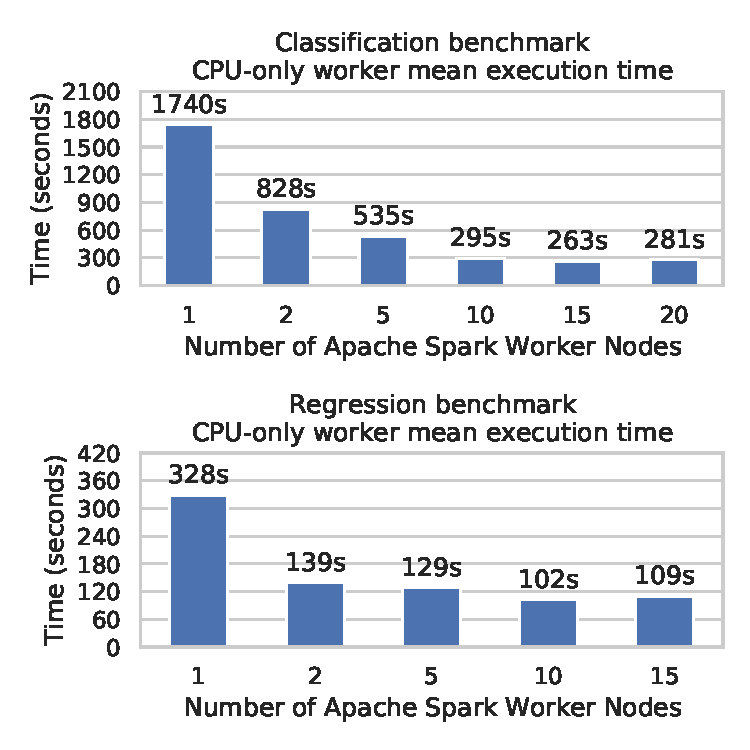
\includegraphics[scale=0.9]{images/07_evaluation/overall_cpu}
\caption{Mean execution time using CPU-only worker nodes}
\label{fig:07_static_results}
\end{figure}
% Explain fig
\Fig{fig:07_static_results} illustrates the mean execution time of both benchmarks for different numbers of worker nodes.
% classification
The best performance for the classification benchmark was achieved with 247 seconds using 30 workers with an improvement of 7.04x compared to 1 worker.
% regression
The regression benchmark performed best with 102 seconds using 10 workers with an improvement of 3.21x in comparison to 1 worker. It achieved a mean execution time of 102 seconds with 30 workers as well. However, using 10 workers is considered the best result for the regression benchmark because fewer workers are used.

\paragraph{}
% The improvement curve
In addition, \Fig{fig:07_static_results} shows that from a specific number of workers onwards, no significant improvement is made.
% Classification
For the classification benchmark, this point is reached at 15 workers.
% Regression
A similar result can be seen for the regression benchmark. From 10 workers onward, the execution time does not improve anymore.
% and?
This result shows that over-provisioning the Apache Spark cluster by simply adding more workers does not improve the performance.


% ===========================================
% ===========================================
\section{GPU-Accelerated Workers}
\label{sec:07_gpu}
% Intro
The impact of \hyperlink{abbr:gpu}{GPU}-accelerated Apache Spark worker nodes for both benchmarks have been evaluated using 2 configurations: Using one and two \hyperlink{abbr:gpu}{GPU}-accelerated worker nodes respectively.
%
The GPU-experiment performance data for the classification benchmark is available in \Fig{fig:appendix_eval_classification_gpu1}, and \Fig{fig:appendix_eval_classification_gpu2}., for the regression benchmark at \Fig{fig:appendix_eval_regression_gpu1}, and \Fig{fig:appendix_eval_regression_gpu2}.


% vs figure
\begin{figure}[h]
\centering
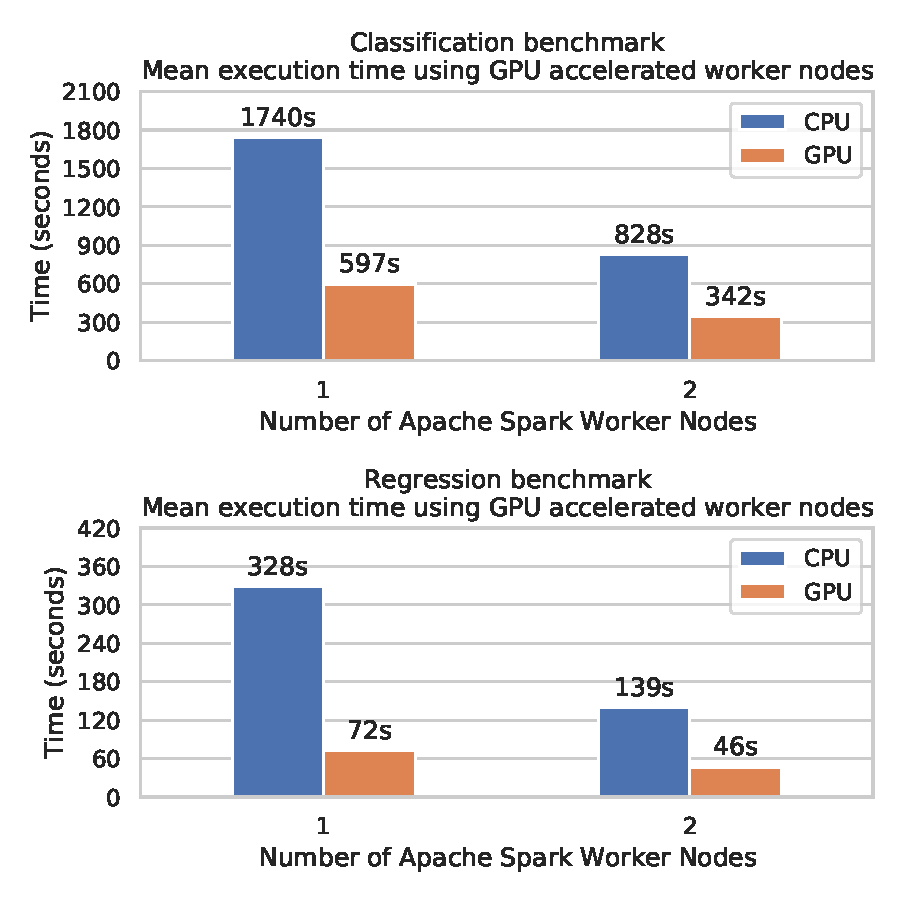
\includegraphics[scale=0.9]{images/07_evaluation/overall_cpu_vs_gpu}
\caption{Mean execution time of GPU-accelerated worker nodes vs. Mean execution time of CPU-only worker nodes}
\label{fig:07_gpu_results}
\end{figure}
% Explain results
The results of the experiment are illustrated in \Fig{fig:07_gpu_results}.
% vs
The mean execution times using \hyperlink{abbr:gpu}{GPU}-accelerated worker nodes are plotted against the mean execution times using \hyperlink{abbr:cpu}{CPU}-only worker nodes.
% overall
Overall, \hyperlink{abbr:gpu}{GPU}-accelerated worker nodes significantly outperformed the equivalent number of \hyperlink{abbr:cpu}{CPU}-only worker nodes.
% classification
For the classification benchmark, the best execution time was achieved using 2 \hyperlink{abbr:gpu}{GPU}-accelerated worker nodes with an improvement of 2.42x compared to 2 \hyperlink{abbr:cpu}{CPU}-only worker nodes. Using 1 \hyperlink{abbr:gpu}{GPU}-accelerated worker node achieved an improvement of 2.91x compared to 1 \hyperlink{abbr:cpu}{CPU}-only worker node.
% regression
The regression benchmark performed best with 2 \hyperlink{abbr:gpu}{GPU}-accelerated worker nodes improving the execution by 3.02x in comparison to 2 \hyperlink{abbr:cpu}{CPU}-only worker nodes. Using 1 \hyperlink{abbr:gpu}{GPU}-accelerated worker node achieved an improvement of 4.55x in comparison to 1 \hyperlink{abbr:cpu}{CPU}-only worker node.

\paragraph{}
% The table
\Tab{table:07_gpu_overall_results} shows the overall results by comparing \hyperlink{abbr:cpu}{CPU}-only and \hyperlink{abbr:gpu}{GPU}-accelerated results for each benchmark.
% classification
For the classification benchmark, 5 \hyperlink{abbr:cpu}{CPU}-only worker nodes outperformed 1 \hyperlink{abbr:gpu}{GPU}-accelerated worker node, and 10 \hyperlink{abbr:cpu}{CPU}-only worker nodes performed better than 2 \hyperlink{abbr:gpu}{GPU}-accelerated worker nodes.
% regression
However, for the regression benchmark, \hyperlink{abbr:cpu}{CPU}-only worker nodes could not outperform \hyperlink{abbr:gpu}{GPU}-accelerated worker node performance.
% Results as table
\begin{table}[ht]
\centering
\begin{tabular}{@{}l|ll|ll@{}}
\toprule
                  & \multicolumn{2}{c|}{Classification}                & \multicolumn{2}{c}{Regression}                    \\
Number of workers & \multicolumn{1}{c}{CPU} & \multicolumn{1}{c|}{GPU} & \multicolumn{1}{c}{CPU} & \multicolumn{1}{c}{GPU} \\ \midrule
1  & 1740s         & 597s          & 328s          & 72s \\
2  & 828s          & \textbf{342s} & 139s          & \textbf{46s} \\
5  & 535s          & -             & 129s          & -     \\
10 & 295s          & -             & \textbf{102s} & -     \\
15 & 263s          & -             & 109s          & -     \\
20 & 281s          & -             & 120s          & -     \\
25 & 257s          & -             & 129s          & -     \\
30 & \textbf{247s} & -             & 102s          & -     \\
35 & 258s          & -             & 109s          & -     \\ \bottomrule
\end{tabular}
\caption{Mean execution time of all CPU-only and GPU-accelerated experiments for both benchmarks}
\label{table:07_gpu_overall_results}
\end{table}


% ===========================================
% ===========================================
\section{Auto-Scaler}
\label{sec:07_auto-scaler}
% Intro
To test the impact of the \textit{Auto-Scaler} while training machine learning applications, both benchmarks have been tested with different \textit{Auto-Scaler} configurations.
% Performance metric
The performance data for the classification benchmark is available in \Fig{fig:appendix_eval_classification_auto-scaler}, and for the regression benchmark in \Fig{fig:appendix_eval_regression_auto-scaler}.


\subsection{Auto-Scaler Benchmark Configurations}
% Wheres it from
The configuration parameters are chosen according to the results of the static worker experiment (\Sec{sec:07_static}).
% Table
The \textit{Auto-Scaler} configuration parameters for each benchmark are shown in \Tab{table:07_auto-scaler_config_parameter}.
% Iteration Figure
\begin{figure}[h]
\centering
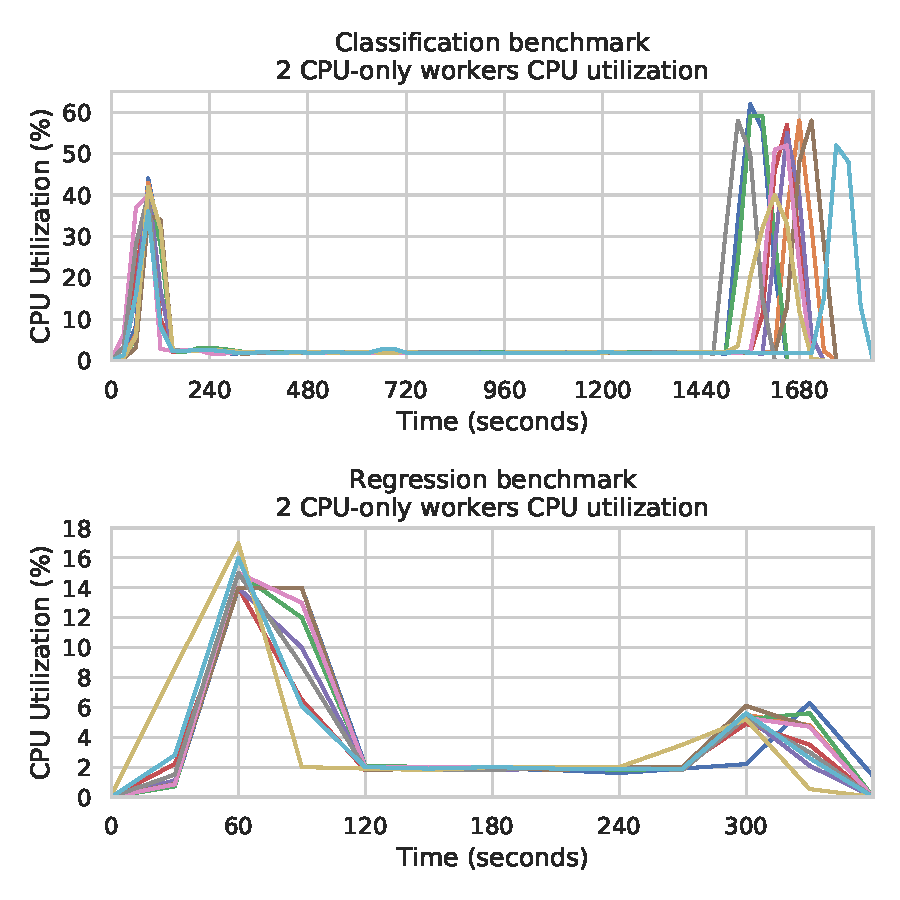
\includegraphics[scale=0.9]{images/07_evaluation/overall_auto-scaler_iterations}
\caption{CPU utilization during all iterations of both benchmarks with 2 CPU-only workers}
\label{fig:07_auto-scaler_iterations_results}
\end{figure}
% Max worker
To prevent cluster over-provisioning, the maximum number of worker nodes for the classification benchmark is set to 15, and 10 for the regression benchmark respectively.
% recurrence
\Fig{fig:07_auto-scaler_iterations_results} shows all 10 iterations of the \hyperlink{abbr:cpu}{CPU}-only experiment for both benchmarks. It shows that, while the machine learning model is trained, only 2 performance spikes occurred at the beginning and at the end during a short period. To scale while these performance spikes occur, the recurrence factor is set to 1. Additionally, the maximum \hyperlink{abbr:cpu}{CPU} utilization for both benchmarks is set according to the maximum \hyperlink{abbr:cpu}{CPU} utilization during the performance spikes.
% The configurations
\begin{table}[ht]
\centering
\begin{tabular}{@{}l|ll@{}}
\toprule
Parameter               & Classification & Regression \\ \midrule
Interval                & 5 seconds      & 5 seconds  \\
Recurrence factor       & 1              & 1          \\
Cooldown period         & 60 seconds     & 60 seconds \\
Target CPU utilization  & 10\%           & 5\%        \\
Minimum CPU utilization & 5\%            & 2\%       \\
Maximum CPU utilization & 25\%           & 10\%       \\
Minimum worker nodes    & 2              & 2         \\
Maximum worker nodes    & 15             & 10         \\ \bottomrule
\end{tabular}
\caption{\textit{Auto-Scaler} configuration parameters for both benchmarks}
\label{table:07_auto-scaler_config_parameter}
\end{table}

\newpage
\subsection{Execution Time Evaluation}
% Figure
\Fig{fig:07_auto-scaler_results} illustrates the results of the \textit{Auto-Scaler} experiment. The mean execution time of 2 \hyperlink{abbr:cpu}{CPU}-only worker nodes is plotted against the mean execution with the \textit{Auto-Scaler} enabled.
% Explain
The results show that no improvement was achieved using the \textit{Auto-Scaler} implementation.
% Results
For the classification benchmark, the execution time increased by 228 seconds when enabling the \textit{Auto-Scaler} in comparison to 2 \hyperlink{abbr:cpu}{CPU}-only worker nodes. Furthermore, the execution time is 38 seconds higher with \textit{Auto-Scaler} enabled than 2 \hyperlink{abbr:cpu}{CPU}-only worker nodes.
% Figure
\begin{figure}[h]
\centering
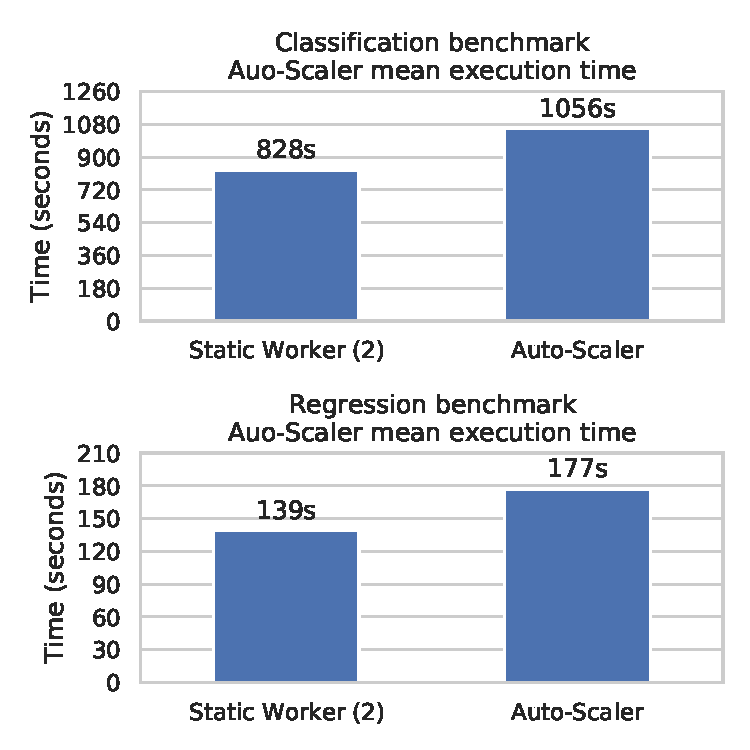
\includegraphics[scale=0.9]{images/07_evaluation/overall_auto-scaler}
\caption{\textit{Auto-Scaler} experiment mean execution time of both benchmarks}
\label{fig:07_auto-scaler_results}
\end{figure}

\newpage
\paragraph{}
% Table
\begin{table}[ht]
\centering
\begin{tabular}{@{}l|ll|ll@{}}
\toprule
                               & \multicolumn{2}{c|}{Classification}                   & \multicolumn{2}{c}{Regression}                       \\
\multicolumn{1}{c|}{Iteration} & \multicolumn{1}{c}{Time} & \multicolumn{1}{c|}{Nodes} & \multicolumn{1}{c}{Time} & \multicolumn{1}{c}{Nodes} \\ \midrule
1  & \textbf{840s} & 15 & 168s          & 5 \\
2  & 960s          & 7  & \textbf{150s} & 2 \\
3  & 1020s         & 15 & 186s          & 6 \\
4  & 1140s         & 15 & 180s          & 6 \\
5  & 1080s         & 15 & 180s          & 6 \\
6  & 1140s         & 15 & 180s          & 6 \\
7  & 1140s         & 15 & 180s          & 6 \\
8  & 1080s         & 15 & 180s          & 6 \\
9  & 1140s         & 7  & 180s          & 6 \\
10 & 1020s         & 15 & 186s          & 6 \\ \bottomrule
\end{tabular}
\caption{Results of each iteration during the \textit{Auto-Scaler} experiment for both benchmarks}
\label{table:07_auto-scaler_iterations}
\end{table}
% Explain
\Tab{table:07_auto-scaler_iterations} summarizes the results for all 10 iterations of each benchmark.
% classification
For the classification benchmark, the best result was achieved in the first iteration with an execution time of 960 seconds and a maximum number of 15 worker nodes during the execution.
% regression
The regression benchmark performed best in the second iteration, with an execution time of 150 seconds and a maximum number of 2 worker nodes during this iteration.
% n maximum reached
The results show that, during the classification benchmark, the \textit{Auto-Scaler} scaled upon the maximum number of allowed worker nodes in 8 out of 10 iterations. During the regression benchmark experiment, the maximum number of worker nodes was never reached. Furthermore, in the second iteration, the \textit{Auto-Scaler} had not scaled the number of worker nodes when the best result was achieved.


\section{Experimental Results Summary}
% Intro
Overall, three different experiments have been conducted to evaluate the implementation of this thesis.
% First experiment
The results of the first experiment show that over-provisioning the Apache Spark cluster does not improve the performance significantly and can negatively impact the performance. 
%  Second
The second experiment shows that \hyperlink{abbr:gpu}{GPU}-accelerated worker nodes significantly outperformed \hyperlink{abbr:cpu}{CPU}-only worker nodes. However, \hyperlink{abbr:cpu}{CPU}-only workers achieved a better performance in the classification benchmark than \hyperlink{abbr:gpu}{GPU}-accelerated workers with 5x the amount.
% Third
For the last experiment, the results show that enabling the \textit{Auto-Scaler} during the training of machine learning models increases the execution time compared with a fixed number of worker nodes.
